\section{Higgs Exotic Decays to Photons and MET Projection Studies}
\subsection{Introduction}

Exotic decays of the Higgs boson can produce the final state consisting of two photons and missing transverse energy (\MET) in different topologies and theoretical benchmarks~\cite{Curtin:2013fra}. 
%
In the non-resonant case, the photons arise from opposite sides of the initial two-body decay: $h\to XX, X\to\gamma Y$, where $Y$ is a stable neutral particle. For instance, such a decay can occur within general gauge mediation models of supersymmetry, in which the $X$ corresponds to a neutralino NLSP with mass less than half the Higgs mass, and the $Y$ corresponds to a gravitino LSP~\cite{Djouadi:1997gw, Mason:2009qh, Petersson:2012dp}.
%
In the resonant case, the photons are produced through an intermediate resonance: $h\to S_1 S_2$, with $S_1 \to\gamma\gamma$ on one side of the decay, while $S_2$ escapes detection, appearing as \MET in the detector. The resonant signal benefits from a peak in the diphoton invariant mass spectrum. 
The Feynman diagrams for the non-resonant and resonant decays can be seen in Figure~\ref{fig:FEYN_SIG}.

Previous searches for the $\gamma\gamma+\MET$ final state in the low energy regime include searches for the non-resonant decay in the supersymmetric scenario described above. CMS and ATLAS have set upper limits on the branching ratio of this decay, with the Higgs boson produced in association with a $Z$ boson \cite{lowmonophoton} and through vector boson fusion \cite{ATLAS:2015bra}.

In this study, we devise a search strategy for the $\gamma\gamma+\MET$ final state, motivated by the exotic decays of the Higgs described above. We estimate the sensitivity of this search for $100$ fb$^{-1}$ of $\sqrt{s}=14$ TeV $pp$ data from the LHC.


%%
\begin{figure}[htbp]
\centering
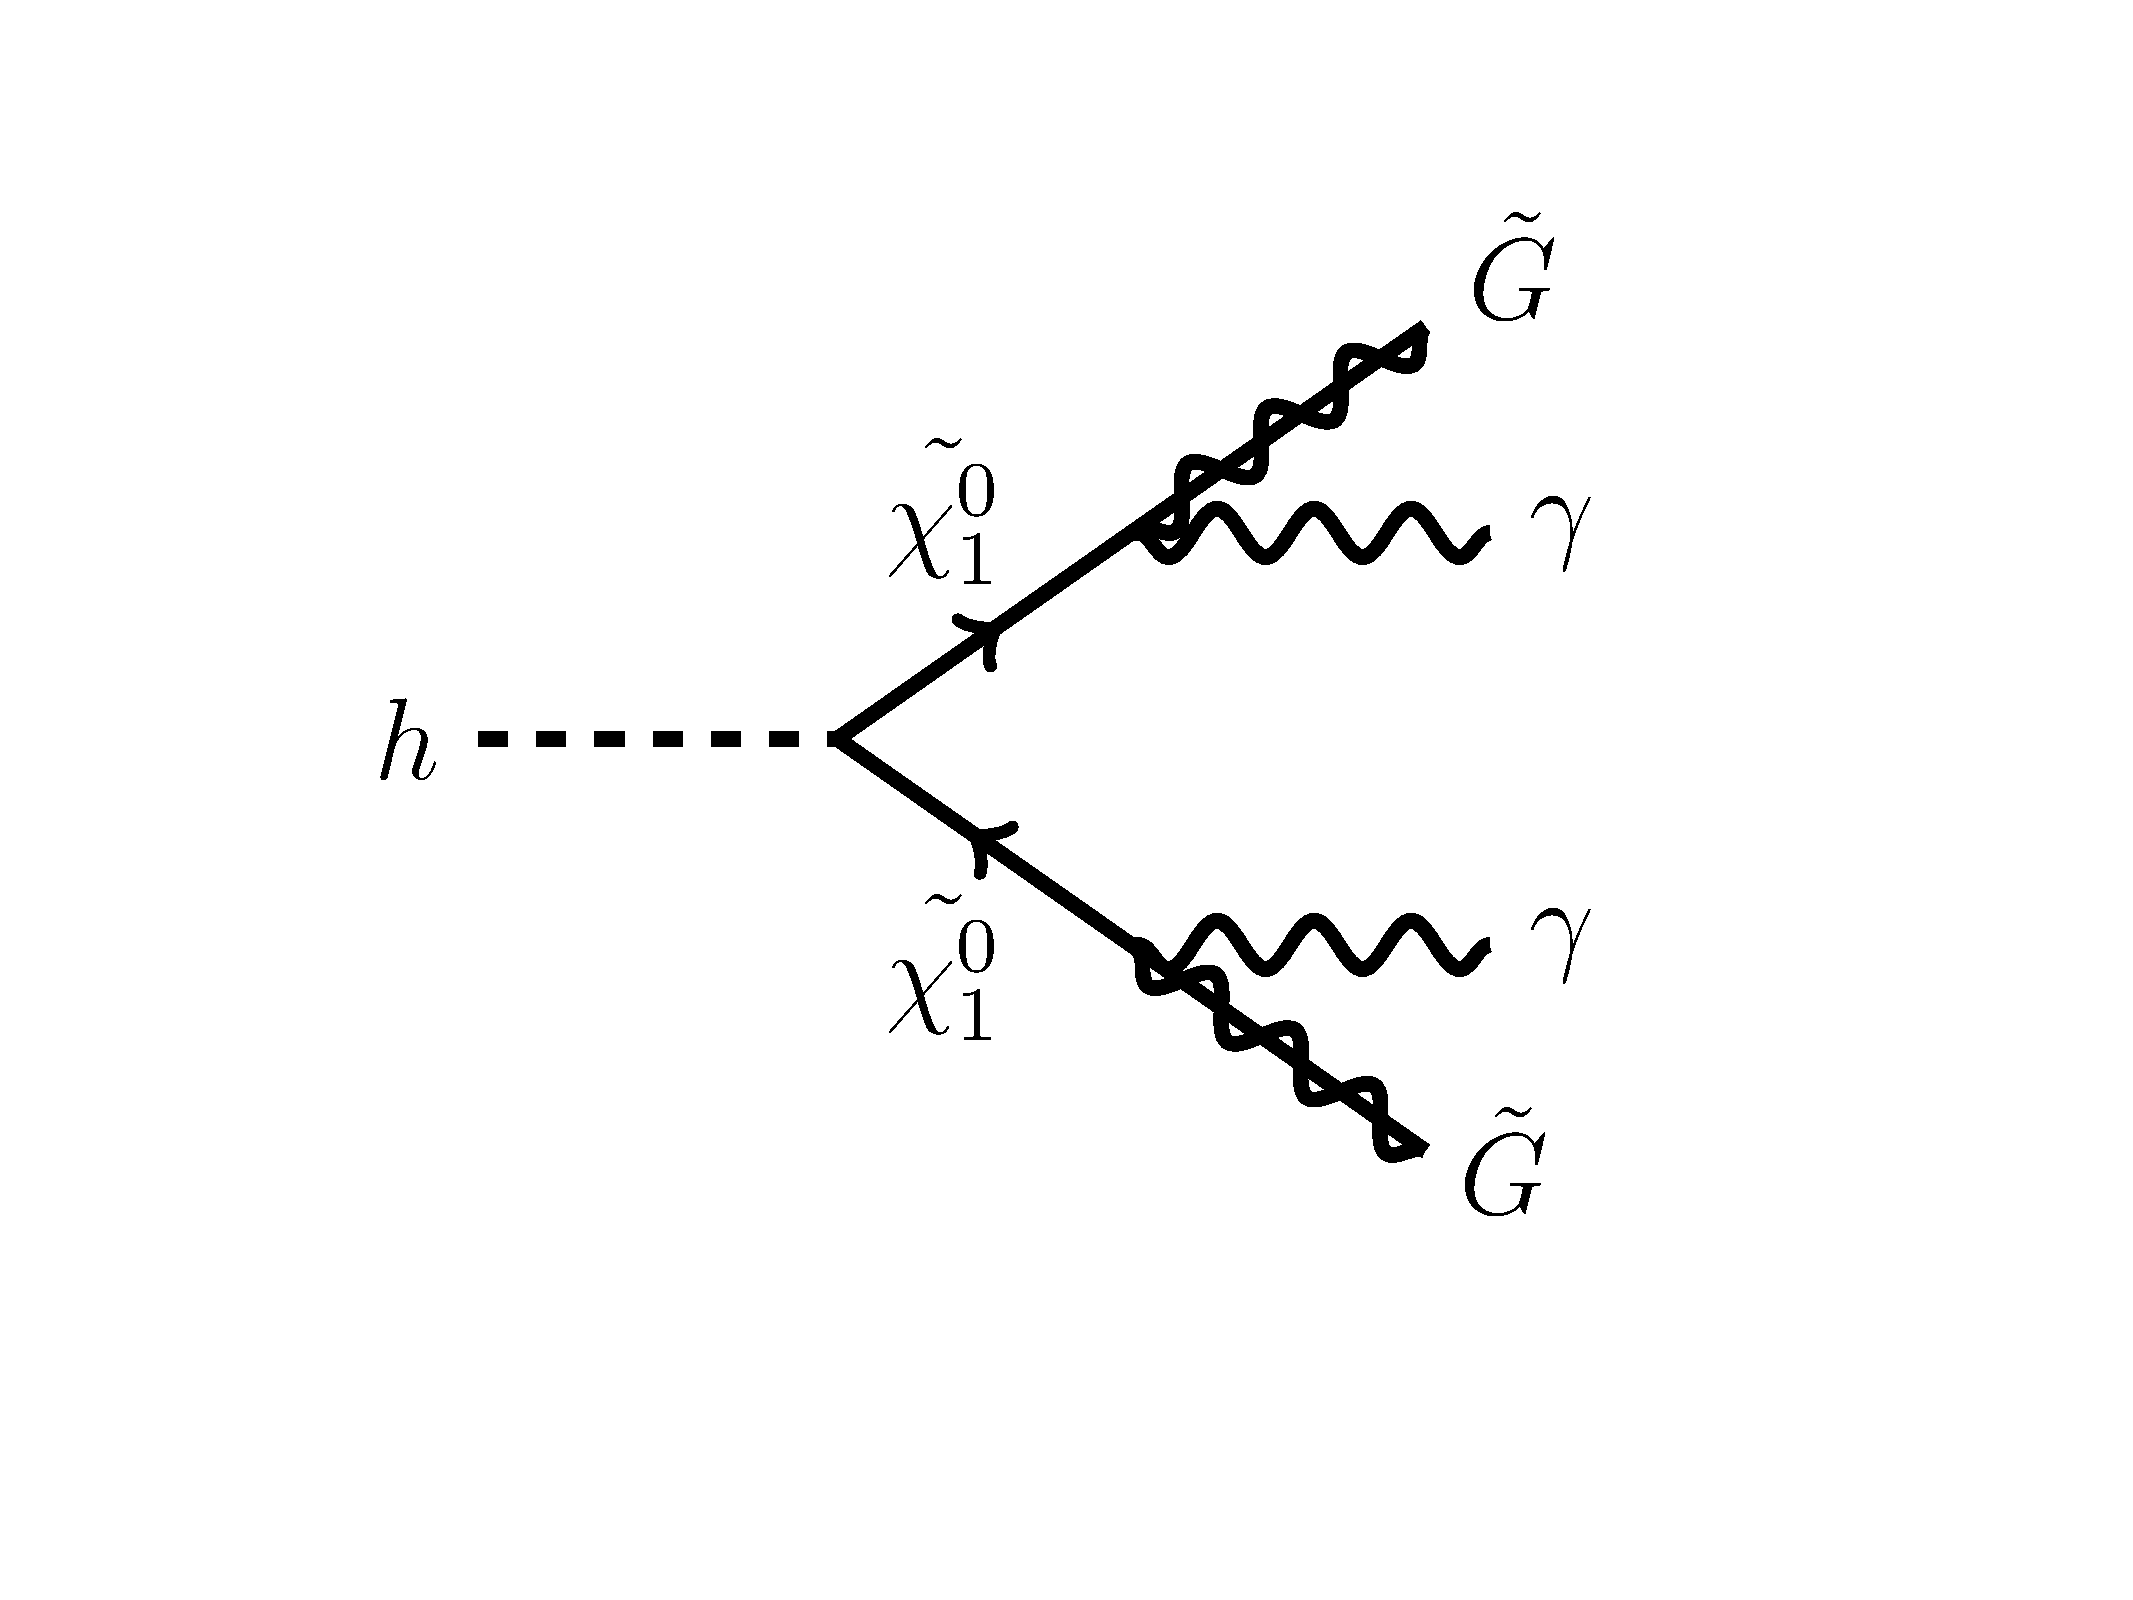
\includegraphics[scale=0.2]{figs/feyn/feyn_nonres.pdf}
\hspace{1cm}
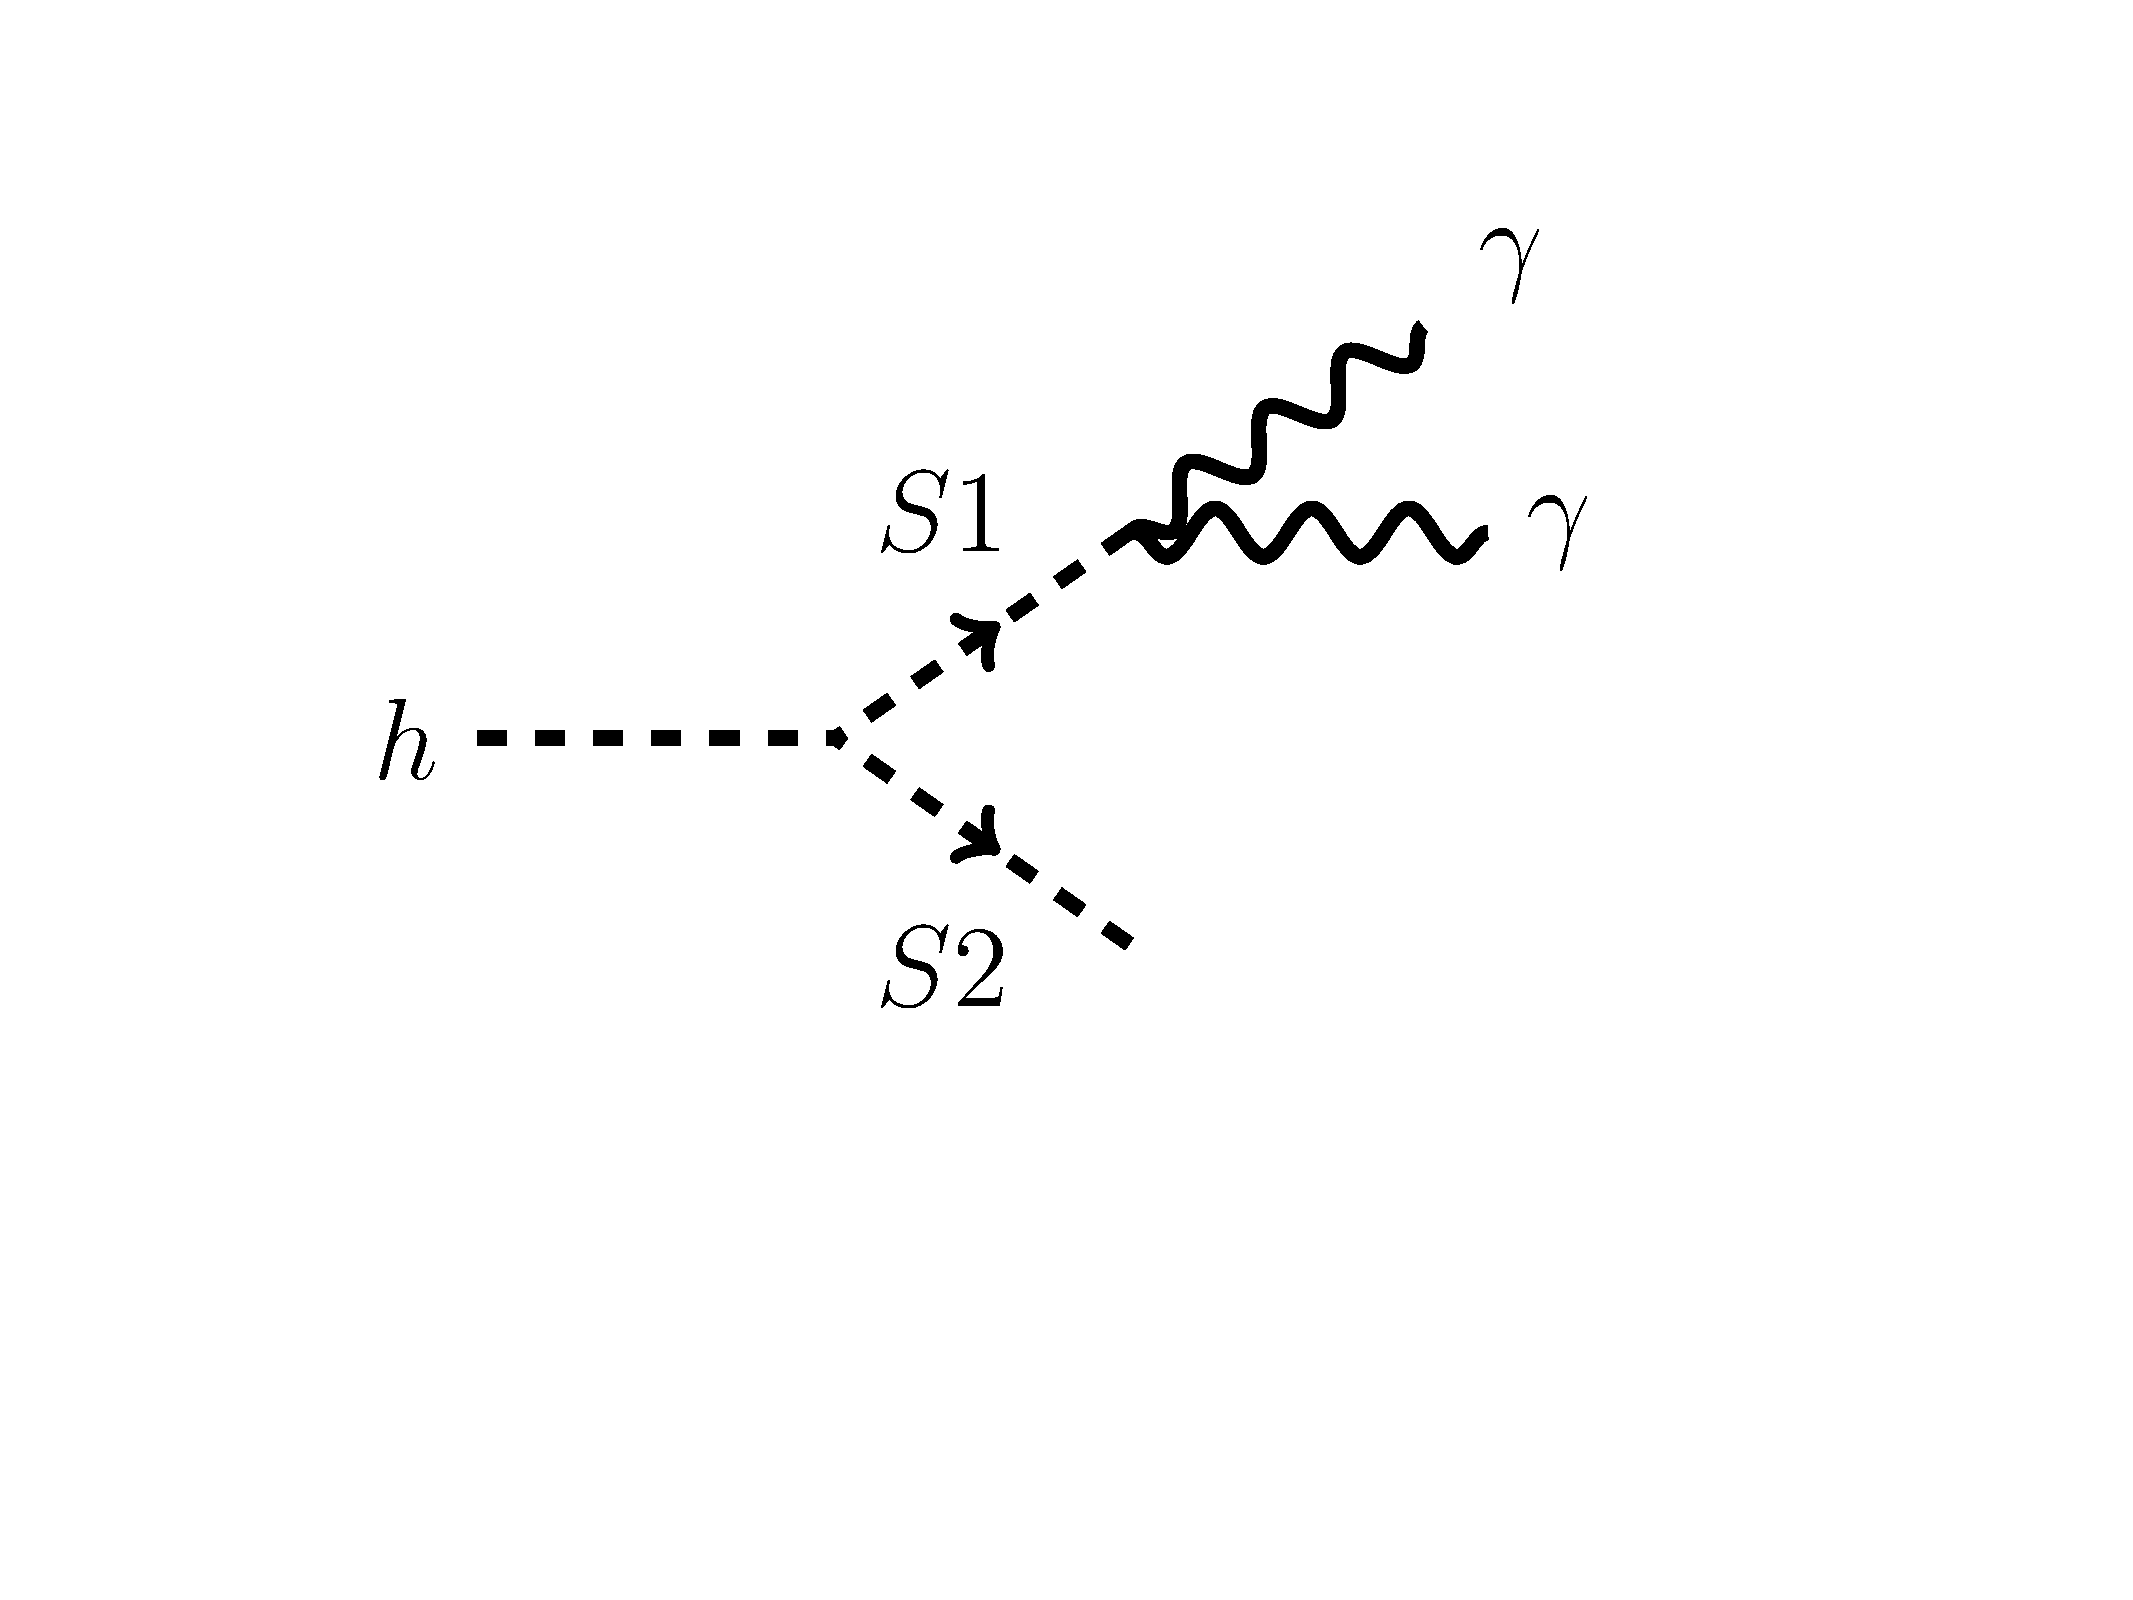
\includegraphics[scale=0.2]{figs/feyn/feyn_res.pdf}
\caption{Feynman diagrams for the (left) the non-resonant and (right) resonant signal scenarios.}
\label{fig:FEYN_SIG}
\end{figure}

\subsection{Methodology}
\subsubsection{Simulation Samples \label{sub:simulation}}

Signal and background Monte Carlo (MC) samples were generated with Madgraph 5~\cite{madgraph} and hadronized with PYTHIA 8~\cite{pythia}, with the detector simulation provided by DELPHES 3~\cite{delphes}.
%The detector card used in DELPHES was based on the CMS detector card, but updated to currently used parameters, such as isolation cone sizes and jet algorithm parameters.
The samples were produced at $\sqrt{s} = 14$ TeV.

The object reconstruction and identification are performed with DELPHES, according to the information provided in the detector configuration card. For the photons reconstruction and identification, we assume an efficiency of $95\%$ in the electromagnetic calorimeter barrel ($|\eta| < 1.5$) and $85\%$ in the endcap ($1.5 < |\eta| < 2.5$). We also impose an isolation cut on the photons by requiring all particle flow candidates within a cone of $\Delta R < 0.3$ to have an energy ratio less than 0.1 with respect to the photon candidate. For muons, we assume an efficiency of $95\%$ for the whole detector acceptance ($|\eta| < 2.5$). An isolation cut similar to the photons is also applied. Jets are reconstructed with the anti-$k_T$ algorithm with $R = 0.4$, similar to the Run 2 analyses at CMS.

\vspace{0.2cm} \textbf{Signal MC Samples}

The signal for the non-resonant case was based on the supersymmetric cascade decay of the Higgs boson into two neutralinos, which subsequently decay into two gravitinos and two photons (Figure \ref{fig:FEYN_SIG}, left). This class of models has been implemented in FeynRules \cite{Christensen:2013aua} and generated via Madgraph 5. We assume a gravitino mass close to zero, which is consistent with gauge mediated low-scale SUSY breaking models with $\sqrt{f} \approx$ TeV \cite{Petersson:2012dp}. We simulate neutralino masses in the range $[10,60]$ GeV in steps of $5$ GeV, with 100,000 events per mass point.

For the resonant case, we assume the Higgs boson decays into two scalar particles, $S_1$ and $S_2$ (Figure \ref{fig:FEYN_SIG}, right). One of the scalars then decays into two photons, while the other escapes detection. For this study, we assume the masses of these two particles are the same; this choice was made for simplicity, but for detailed studies, more combinations should be investigated. We generate samples with $M_{1} = M_{2} = [10,60]$ GeV, in steps of $5$ GeV, with 100,000 events per mass point.

We investigate the production of the Higgs boson through both gluon fusion and associated production with a $Z$ boson ($ZH$), with the $Z$ boson decaying to two muons. The inclusion of the dielectron decay of the $Z$ can also be considered for future studies.
%As such, the signal production cross subsection
%
A branching ratio of ${B}(H\to\gamma\gamma+\MET) = 10\%$ is assumed for the signal. This value of the branching ratio was chosen to be within the current bounds on the Higgs boson width, yet close to the 8 TeV limits from the search for Higgs decays to the monophoton final state ($H\to\gamma+\MET$)~\cite{lowmonophoton}, when combining gluon fusion and ZH production mechanisms.


\vspace{0.2cm} \textbf{Background MC Samples}

Although this analysis is not guaranteed to be entirely free from QCD multi-jet backgrounds, it has been shown in similar analyses (such as \cite{lowmonophoton}) that it is possible to reduce the QCD to a sub-dominant contribution. As such, the remaining backgrounds for this analysis arise predominantly from the single boson ($\gamma$/$Z$/$W$) plus jets and diboson processes.

The background samples were modeled using the Snowmass LHE simulation samples~\cite{Anderson:2013kxz}. They consist of single boson samples ($\gamma/Z/W$) with at least one jet and inclusive diboson ($\gamma\gamma/Z\gamma/W\gamma/$ $WW/ZZ/WZ$) samples. No pure QCD sample was produced for this study. The samples include both hadronic and leptonic decays of the $W$ and $Z$ bosons. The cross subsections used for normalizing the single boson samples were estimated with MCFM~\cite{MCFM}, assuming an efficiency of $15\%$ for the 1 jet requirement (obtained with Madgraph). For the diboson samples, the cross subsections used were estimated from the reference \cite{Campbell:2011bn}. The cross subsections and number of events in the samples are shown in Table \ref{tab:sel_eff}.


\subsubsection{Event Selection}

\vspace{0.2cm} \textbf{Trigger Projections}

For the $ZH$ channel, the trigger strategy is expected to be straightforward and can be based on the decay of the $Z$ to two muons.
%
%The trigger projections for the ZH channel should be straightforward, given its use of the leptonic decay of the Z boson for triggering. Triggering on the Z boson is a safe assumption, since it's used for several physics analysis, including Standard Model Higgs searches and measurements.
%
On the other hand, triggering is one of the main challenges for the gluon fusion channel, since the final state consists of two soft photons plus missing energy. The standard triggers used for $H\rightarrow\gamma\gamma$ analyses typically have a diphoton invariant mass cut which makes it incompatible with the low energy spectrum of this analysis. However, we have identified three possible trigger strategies for this channel, based on  unprescaled triggers used by the CMS experiment in Run-2:

\begin{itemize}
\item Asymmetric Diphoton Trigger: This trigger requires two photons with different $E_{T}$ and trigger-level identification requirements, plus a diphoton invariant mass cut. This type of trigger usually has a non-negligible turn-on curve in the leading and subleading photon  $E_{T}$.
\item Symmetric Diphoton Trigger: This trigger requires two photons with the same $E_{T}$ requirement, without any extra requirement.
\item $\gamma+\MET$ Trigger: This trigger requires only one barrel photon passing identification requirements and a $E_{T}$ requirement that is usually higher than the previous two triggers. In addition, there is a calorimetric \MET requirement. We expect non-negligible turn-on curves with respect to both photon and \MET for this trigger.
\end{itemize}

The three triggers described here represent different selection strategies that were investigated and will be described below.


\vspace{0.2cm} \textbf{Offline Selection}

The gluon fusion selection is based on the diphoton selection and must reflect the chosen trigger strategy, while maintaining a good signal efficiency. 
%The final selections for each trigger scenario investigated are shown in Table \ref{tab:sel_ggh}.
%
%\begin{table}[]
%\centering
%\begin{tabular}{| r | l | l | l|}
%\hline
%Variable & Asymmetric Diphoton & Symmetric Diphoton & %\gamma+\MET \\ \hline
%Number of photons & $> 1$ & $> 1$ & $> 1$ \\
%$p_{T}(\gamma_{1})$ & $ > 45$ GeV & $ > 40$ GeV & $ > 55$ GeV \\
%$|\eta(\gamma_{1})|$ & $ < 2.5 & $ < 2.5 & $ < 1.4 \\
%$p_{T}(\gamma_{2})$ & $ > 30$ GeV & $ > 40$ GeV & $ > 15$ GeV \\
%$|\eta(\gamma_{2})|$ & $ < 2.5 & $ < 2.5 & $ < 2.5 \\
%$M(\gamma\gamma)$ & $< 100$ GeV & $< 100$ GeV & $< 100$ GeV \\
%$M(\gamma\gamma)$ & $> 15$ GeV & - & - \\
%$\MET$ & $> 40$ GeV & $> 40$ GeV & $> 50$ GeV\\
%\hline
%\end{tabular}
%\caption{Analysis selection for the gluon fusion channel, for each trigger scenario.}
%\label{tab:sel_ggh}
%\end{table}
%
%\vspace{0.2cm} \textbf{Selection: $ZH$ Channel}
%
The $ZH$-produced signal events are tagged through the decay of the $Z$ boson to muons, minimizing the largest backgrounds. 
%so the starting point is the selection of two well isolated muons peaking around the $Z$ mass. 
The photon selection is chosen to maximize the signal acceptance in the $ZH$ case, with $E_{T}$ thresholds as low as possible. 
%The final $ZH$ event selection is show in Table \ref{tab:sel_zh}.
%
The final event selection requirements for the gluon fusion  and $ZH$ channels are summarized in Table~\ref{tab:sel_all}. On this table, we use the following definitions for transverse mass:
%\begin{equation}
\begin{align}
M_{T}(\gamma\gamma,\MET) &= \sqrt{2E_{T}(\gamma\gamma)\MET(1-\cos(\Delta\phi(\gamma\gamma,\MET))}, \\
M_{T}(\gamma\gamma+\MET, \mu\mu) &= \sqrt{2E_{T}(\gamma\gamma+\MET)p_{T}(\mu\mu)(1-\cos(\Delta\phi(\gamma\gamma+\MET,\mu\mu))}.
\end{align}
%\end{equation}

%\begin{table}[]
%\centering
%\begin{tabular}{| r | l|}
%\hline
%Variable & Requirement \\ \hline
%Number of photons & $> 1$ \\
%$p_{T}(\gamma_{1,2})$ & $ > 15$ GeV \\
%$|\eta(\gamma_{1,2})|$ & $ < 2.5 \\
%$M(\gamma\gamma)$ & $< 100$ GeV \\
%$\MET$ & $> 40$ GeV \\ 
%Number of muons & $> 1$ \\
%$p_{T}(\mu_{1,2})$ & $ > 20$ GeV \\
%$|\eta(\mu_{1,2})|$ & $ < 2.5 \\
%$M(\mu\mu)$ & $\in [70,110]$ GeV\\
%\hline
%\end{tabular}
%\caption{Analysis selection for the $ZH$ channel.}
%\label{tab:sel_zh}
%\end{table}

\begin{table}[]
\centering
\begin{tabular}{| r | l | l | l| l|}
\hline
 & \multicolumn{3}{|c|}{gluon Fusion} & \multicolumn{1}{|c|}{$ZH$} \\ 
\hline
Variable & Asymmetric $\gamma\gamma $& Symmetric $\gamma\gamma$ & $\gamma+\MET$ & \\ \hline
Number of photons       & $> 1$         & $> 1$         & $> 1$         & $> 1$\\
$p_{T}(\gamma_{1})$     & $ > 45$ GeV   & $ > 40$ GeV   & $ > 55$ GeV   & $ > 20$ GeV\\
$|\eta(\gamma_{1})|$    & $ < 2.5$      & $ < 2.5$      & $ < 1.4$      & $< 2.5$ \\
$p_{T}(\gamma_{2})$     & $ > 30$ GeV   & $ > 40$ GeV   & $ > 20$ GeV   & $ > 20$ GeV\\
$|\eta(\gamma_{2})|$    & $ < 2.5$      & $ < 2.5$      & $ < 2.5$      & $ < 2.5$ \\
$M(\gamma\gamma)$       & $\in [15, 100]$ GeV & $< 100$ GeV & $< 100$ GeV & $< 100$ GeV \\
$\MET$                  & $> 90$ GeV    & $> 90$ GeV    & $> 90$ GeV    & $> 60$ GeV \\
$M_{T}(\gamma\gamma,\MET)$                    & $< 140$ GeV   & $< 140$ GeV   & $< 140$ GeV   & $< 140$ GeV \\
$\Delta\phi(\gamma\gamma,\MET)$ & $< 1.5$ & $< 1.5$ & $< 1.5$ & $< 1.5$ \\
Number of leptons       & $< 1$         & $< 1$         & $< 1$         & 2 muons \\
\hline
%Number of muons & - & - & - & $> 1$ \\
$p_{T}(\mu_{1,2})$ & -  & - & - & $ > 20$ GeV \\
$|\eta(\mu_{1,2})|$ & - & - & - & $ < 2.5$ \\
$M(\mu\mu)$ & - & - & - & $\in [75,115]$ GeV\\
$M_{T}(\gamma\gamma+\MET, \mu\mu)$ & - & - & - & $> 400$ GeV\\
\hline
\end{tabular}
\caption{Analysis selection for the gluon fusion channel (for each trigger scenario) and the $ZH$ channel.}
\label{tab:sel_all}
\end{table}

%\begin{table}[]
%\centering
%\begin{tabular}{| r | l | l | l| l|}
%\hline
% & \multicolumn{3}{|c|}{gluon Fusion} & \multicolumn{1}{|c|}{$ZH$} \\ 
%\hline
%Variable & ZH & \\ \hline
%Number of photons    & $> 1$\\
%$p_{T}(\gamma_{1})$  & $ > 20$ GeV\\
%$|\eta(\gamma_{1})|$ & $< 2.5$ \\
%$p_{T}(\gamma_{2})$  & $ > 20$ GeV\\
%$|\eta(\gamma_{2})|$ & $ < 2.5$ \\
%$M(\gamma\gamma)$    & $< 100$ GeV \\
%$\MET$               & $> 60$ GeV \\
%$M_{T}(\gamma\gamma,\MET)$ & $< 140$ GeV \\
%$\Delta\phi(\gamma\gamma,\MET)$ & $< 1.5$ \\
%Number of leptons       & 2 muons \\ \hline
%%Number of muons & $> 1$ \\
%$p_{T}(\mu_{1,2})$ & $ > 20$ GeV \\
%$|\eta(\mu_{1,2})|$ & $ < 2.5$ \\
%$M(\mu\mu)$ & $\in [75,115]$ GeV\\
%$M_{T}(\gamma\gamma+\MET, \mu\mu)$ & $> 400$ GeV\\ \hline
%\end{tabular}
%\caption{Analysis selection for the gluon fusion channel (for each trigger scenario) and the $ZH$ channel.}
%\label{tab:seldas_all}
%\end{table}


To exploit the topology of the resonant signature, we apply an additional requirement of a $\pm10$ GeV mass window, in the diphoton invariant mass distribution ($M(\gamma\gamma)$), around the signal mass ($M_1$). The efficiencies for each individual process and the different searches, after the full selection (without the $M(\gamma\gamma)$ mass window requirement), are shown in Table \ref{tab:sel_eff}.

For the ZH case, we also explore the strategy performed by CMS in their Run I result \cite{lowmonophoton}, in which one or more photons are required in the event, instead of two or more. In this case, we gain back the efficiency that is lost due to the inefficiency in reconstructing the subleading photon, which can have very low $E_T$. The selection is similar to what is described in Table \ref{tab:sel_all}, but without the $M(\gamma\gamma)$ cut or the mass window requirement for the non resonant topology. The other variables that use the diphoton information are instead reconstructed with the leading photon in the event.

\begin{table}[]
\centering
\resizebox{\textwidth}{!}{
\begin{tabular}{| c | c | c | c | c | c| c| }
\hline
 \multirow{ 2}{*}{Process} &  \multirow{ 2}{*}{$\sigma$ (pb)} & \multirow{ 2}{*}{$N_\text{Generated}$} & \multicolumn{3}{|c|}{gluon Fusion} & \multirow{ 2}{*}{$ZH$} \\ 
 & & & Asymmetric $\gamma\gamma$ & Symmetric $\gamma\gamma$ & $\gamma+\MET$ & \\ \hline
\multicolumn{7}{|c|}{Backgrounds} \\
\hline
$\gamma$ + Jets    & $1.0\times10^{5}$  &    5425448    &    $1.9\times10^{-6}$  &   $4.7\times10^{-7}$  &   $8.9\times10^{-7}$  &   $\approx 0$   \\
$Z$ + Jets         & $0.94\times10^{4}$   &    1888446    &  $5.6\times10^{-4}$    & $1.5\times10^{-4}$    & $5.0\times10^{-5}$    & $\approx 0$     \\
$W$ + Jets         & $2.96\times10^{4}$  &    5263872    &   $6.2\times10^{-4}$   &  $1.9\times10^{-4}$   &  $2.7\times10^{-5}$   &  $\approx 0$    \\
$\gamma\gamma$     & $10.8\times10^{1}$  &    4268781    &   $3.1\times10^{-5}$   &  $1.0\times10^{-5}$   &  $1.1\times10^{-5}$   &  $\approx 0$             \\
$Z\gamma$          & $6.30\times10^{2}$  &    3406151    &   $4.3\times10^{-4}$   &  $1.4\times10^{-4}$   &  $5.7\times10^{-5}$   &  $\approx 0$    \\
$W\gamma$          & $1.03\times10^{3}$   &    5258034    &  $1.4\times10^{-4}$    & $4.6\times10^{-5}$    & $5.4\times10^{-5}$    & $\approx 0$     \\
$WW$               & $1.24\times10^{2}$  &    8059829    &   $2.6\times10^{-1}$   &  $8.4\times10^{-2}$   &  $9.8\times10^{-5}$   &  $8.2\times10^{-8}$    \\
$ZZ$               & $1.8\times10^{1}$ &    1101611    &     $1.4\times10^{-2}$ &    $4.7\times10^{-3}$ &    $6.7\times10^{-4}$ &    $7.3\times10^{-6}$ \\
$WZ$               & $5.1\times10^{1}$ &    3319770    &     $3.6\times10^{-1}$ &    $1.2\times10^{-1}$ &    $2.5\times10^{-4}$ &    $2.9\times10^{-6}$  \\

%\hline
%\multicolumn{7}{|c|}{Signals} \\
%\hline
%Res., M = 10 GeV     &  $10.8\times10^{1}$   &    4268781    &  $2.5\times10^{-4}$   &  $2.2\times10^{-4}$   &  $1.7\times10^{-4}$   &  $5.7\times10^{-4}$       \\
%Res., M = 40 GeV     &  $6.30\times10^{2}$   &    3406151    &  $8.7\times10^{-3}$   &  $5.7\times10^{-3}$   &  $5.0\times10^{-3}$   &  $6.9\times10^{-3}$      \\
%Res., M = 60 GeV     &  $1.03\times10^{3}$    &    5258034    & $1.6\times10^{-2}$    & $1.1\times10^{-2}$    & $1.1\times10^{-2}$    & $9.2\times10^{-3}$         \\
%Non-Res., M = 10 GeV &  $1.24\times10^{2}$   &    8059829    &  $1.5\times10^{-3}$   &  $9.5\times10^{-4}$   &  $1.1\times10^{-3}$   &  $1.1\times10^{-3}$       \\
%Non-Res., M = 40 GeV &  $1.8\times10^{1}$  &    1101611    &    $8.0\times10^{-3}$ &    $5.5\times10^{-3}$ &    $5.2\times10^{-3}$ &    $6.3\times10^{-3}$     \\
%Non-Res., M = 60 GeV &  $5.1\times10^{1}$  &    3319770    &    $1.1\times10^{-2}$ &    $7.6\times10^{-3}$ &    $6.9\times10^{-3}$ &    $8.1\times10^{-3}$     \\
\hline
\end{tabular}
}
\caption{Cross subsections, numbers of events generated per process, and selection efficiencies for background processes, for gluon fusion and $ZH$ production mechanisms.}
\label{tab:sel_eff}
\end{table}

\subsubsection{Background Estimation for Misidentified Photons}

Background processes with mis-identified (or "fake") photons, such as jets and electrons misidentified as photons, that pass the final selection generally have very low efficiency at the LHC. Nonetheless, such backgrounds may be non-negligible since the production cross-subsections can be large. Such mis-identification rates are typically measured with data-driven methods at the LHC.
%
%Because of that, it's costumary for analysis involving a large amount of background events with fake objects to estimate those processes with data driven approaches. Otherwise, the amount of MC events needed to have a good description of the background after selection would be too large. 
Although this study was limited by MC statistics in measuring fake photon backgrounds, a method was developed to mitigate this problem, which we describe below.

The object reconstruction and selection is done at DELPHES level, where, given the photon identification requirements described in subsection \ref{sub:simulation}, we obtain an associated fake rate. These fake rates are accounted for in the overall efficiencies in Table \ref{tab:sel_eff}. In order to bypass the efficiency loss due to the small fake rates, we select jets and electrons as fake photon candidates. For the background processes with one prompt photon ($\gamma$+jets, $W\gamma$ and $Z\gamma$), we select one fake photon candidate. For the processes with no prompt photons ($W/Z$+jets, $WW$, $WZ$ and $ZZ$), we select two fake photon candidates. No fake photon selection is done for the $\gamma\gamma$+jets sample.

With the assumption of a flat fake rate for both jets and electrons, the fake photon candidates are randomly selected from the jets and electrons that passed the photon acceptance requirements. One extra assumption is that the electron-to-photon fake rate is set to be order of magnitude larger than the jets-to-photon fake rate. Therefore, electrons are set to have a probability of being selected to be a misidentified photon that is ten times higher than for jets.

After the choice of fake photon candidates, we calculate weights for the individual samples based on the $E_{T}$ spectrum of the selected photons (prompt and fake) to match the spectrum found with the photon candidates reconstructed directly from DELPHES. This reweighting is done on the sum of $E_{T}$ of the two leading photons for samples with at least one prompt photon, and on the $E_{T}$ of the leading photon for samples with no prompt photon. An independent reweighting is also done in $\eta$. Both reweightings reflect the different reconstruction efficiencies and energy resolutions of objects that are not reconstructed as photons. After applying the weights, we observe a good agreement between the kinematic distributions of interest arising from photons reconstructed by DELPHES and from our fake photon candidates.

\subsection{Results}

We present the expected sensitivity of this search in terms of the necessary $h\rightarrow\gamma\gamma+\MET$ branching ratio to reach a $5\sigma$ sensitivity for an assumed integrated luminosity of $100$ fb$^{-1}$ at $\sqrt{s} = 14$ TeV, with the frequentist sensitivity defined as:
%
\begin{equation}
\mathcal{S} = \frac{N_\text{Signal}}{\sqrt{N_\text{Background}}}.
\end{equation}

In Figure \ref{fig:triggers} (left), we shown the signal efficiency for the different trigger selections presented and (right) the sensitivity plot for the gluon fusion case.
%$5\sigma$ branching ratios for the different trigger scenarios in the gluon fusion analysis, in the resonant (left) and non-resonant (right) final states. 
This plot shows that, after the full selection, the performance of the triggers is comparable. Although it's safe to assume that a diphoton trigger with a low $M(\gamma\gamma)$ cut will be present in the future trigger menus of CMS and ATLAS, we choose to perform the analysis in the $\gamma+\MET$ case. We make this choice as an effort to make the case for the existence of such a trigger strategy for the future LHC runs. While the diphoton triggers are designed with specific usages that are already well stablished, the $h\rightarrow\gamma\gamma+\MET$ analysis could be viewed as a benchmark for the $\gamma+\MET$ trigger for three reasons:
\begin{itemize}
    \item It's a trigger that is already present at the LHC experiments, but can be retuned with a specific analysis as benchmark;
    \item A dedicated trigger for this analysis requiring two photons might not be as efficient at trigger legel, given the soft spectrum of the second photon;
    \item This trigger can also be used for other exotic searches, such as the extension to low energies of the dark matter searches in the monophoton channel.
\end{itemize}
%assumption to have the diphoton trigger in the future trigger menus for CMS and ATLAS for different searches that involve low energy diphotons, the \gamma+\MET trigger outperforms the other two possibilities, for both resonant and non-resonant topologies. This is due to the fact that the subleading photon $E_{T}$ requirement can be very low since we trigger on the leading photon and there is no trigger-level requirement on the subleading photon.

\begin{figure}[htbp]
\centering
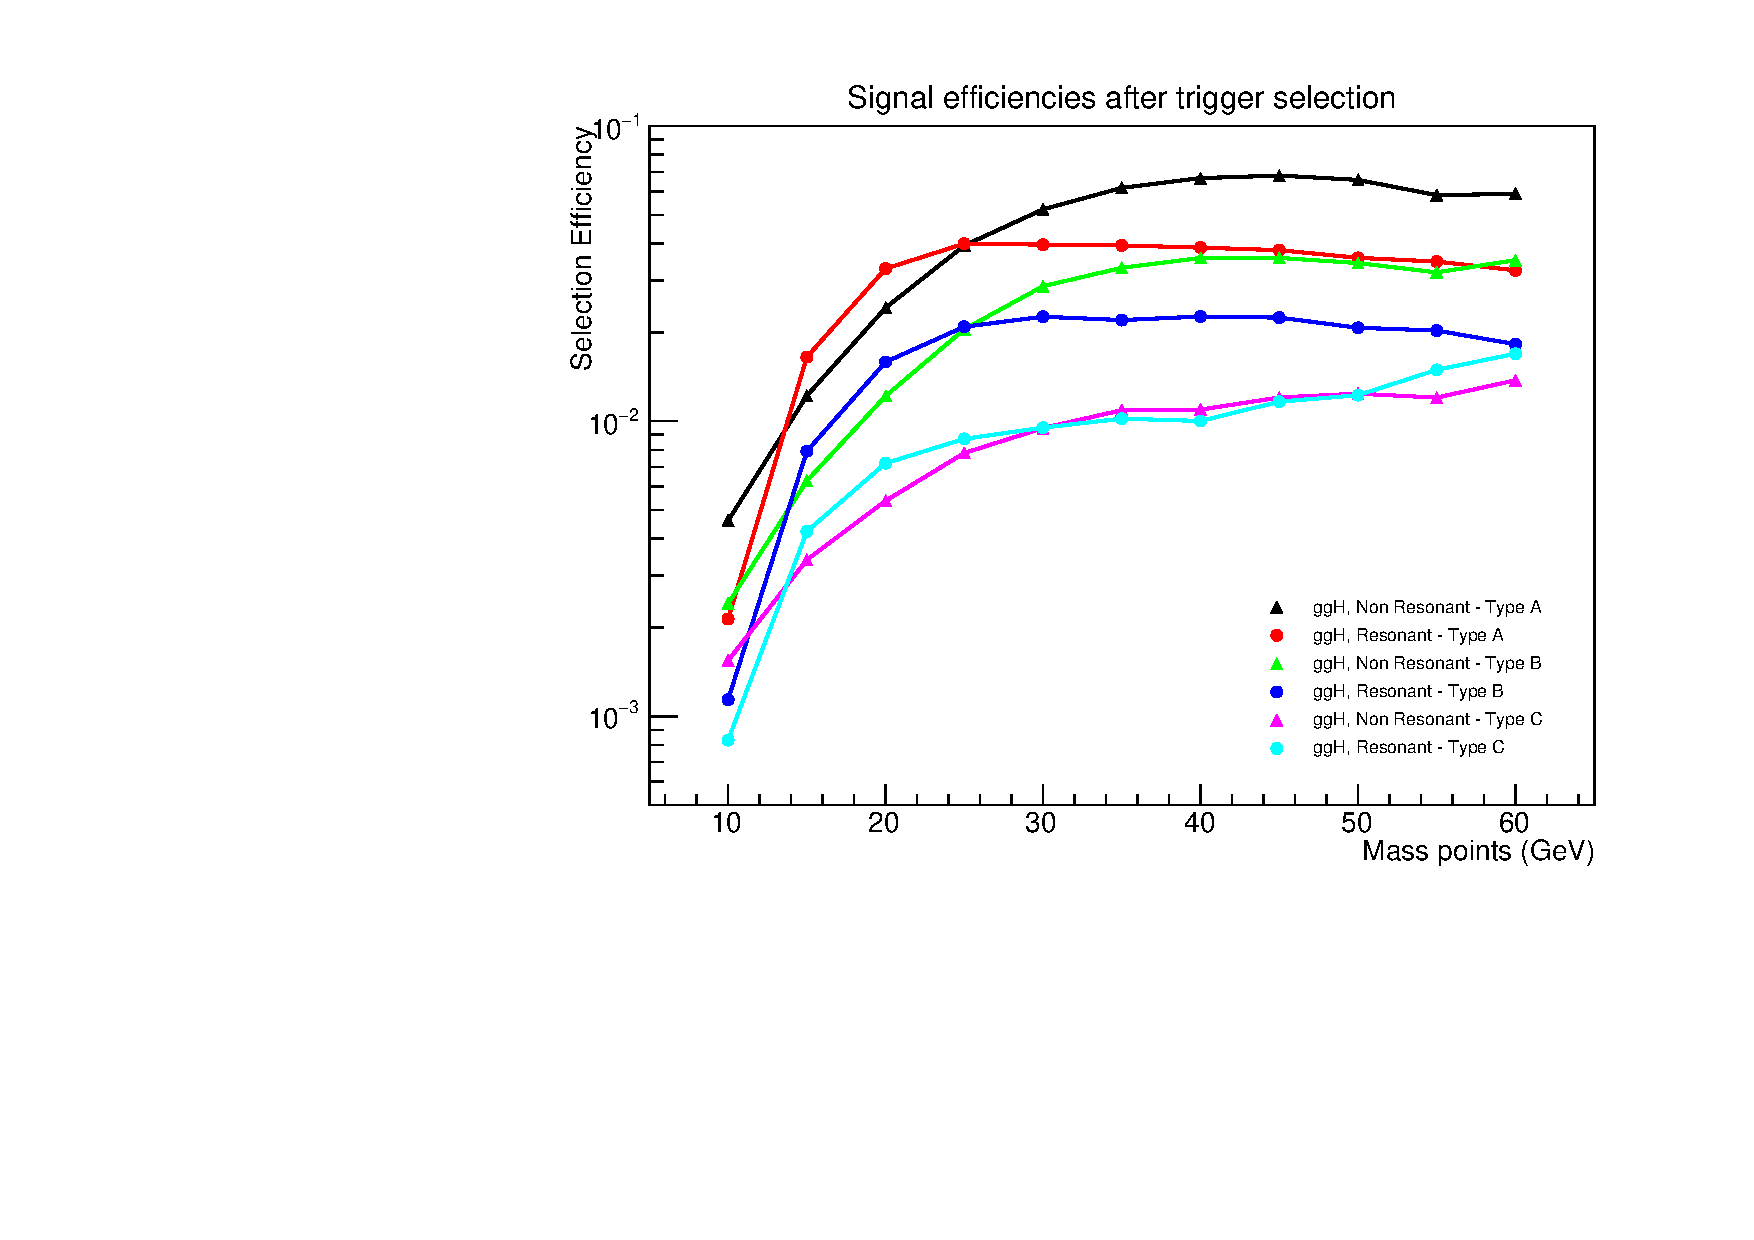
\includegraphics[width=0.45\textwidth]{triggerplots/Efficiencies.pdf}
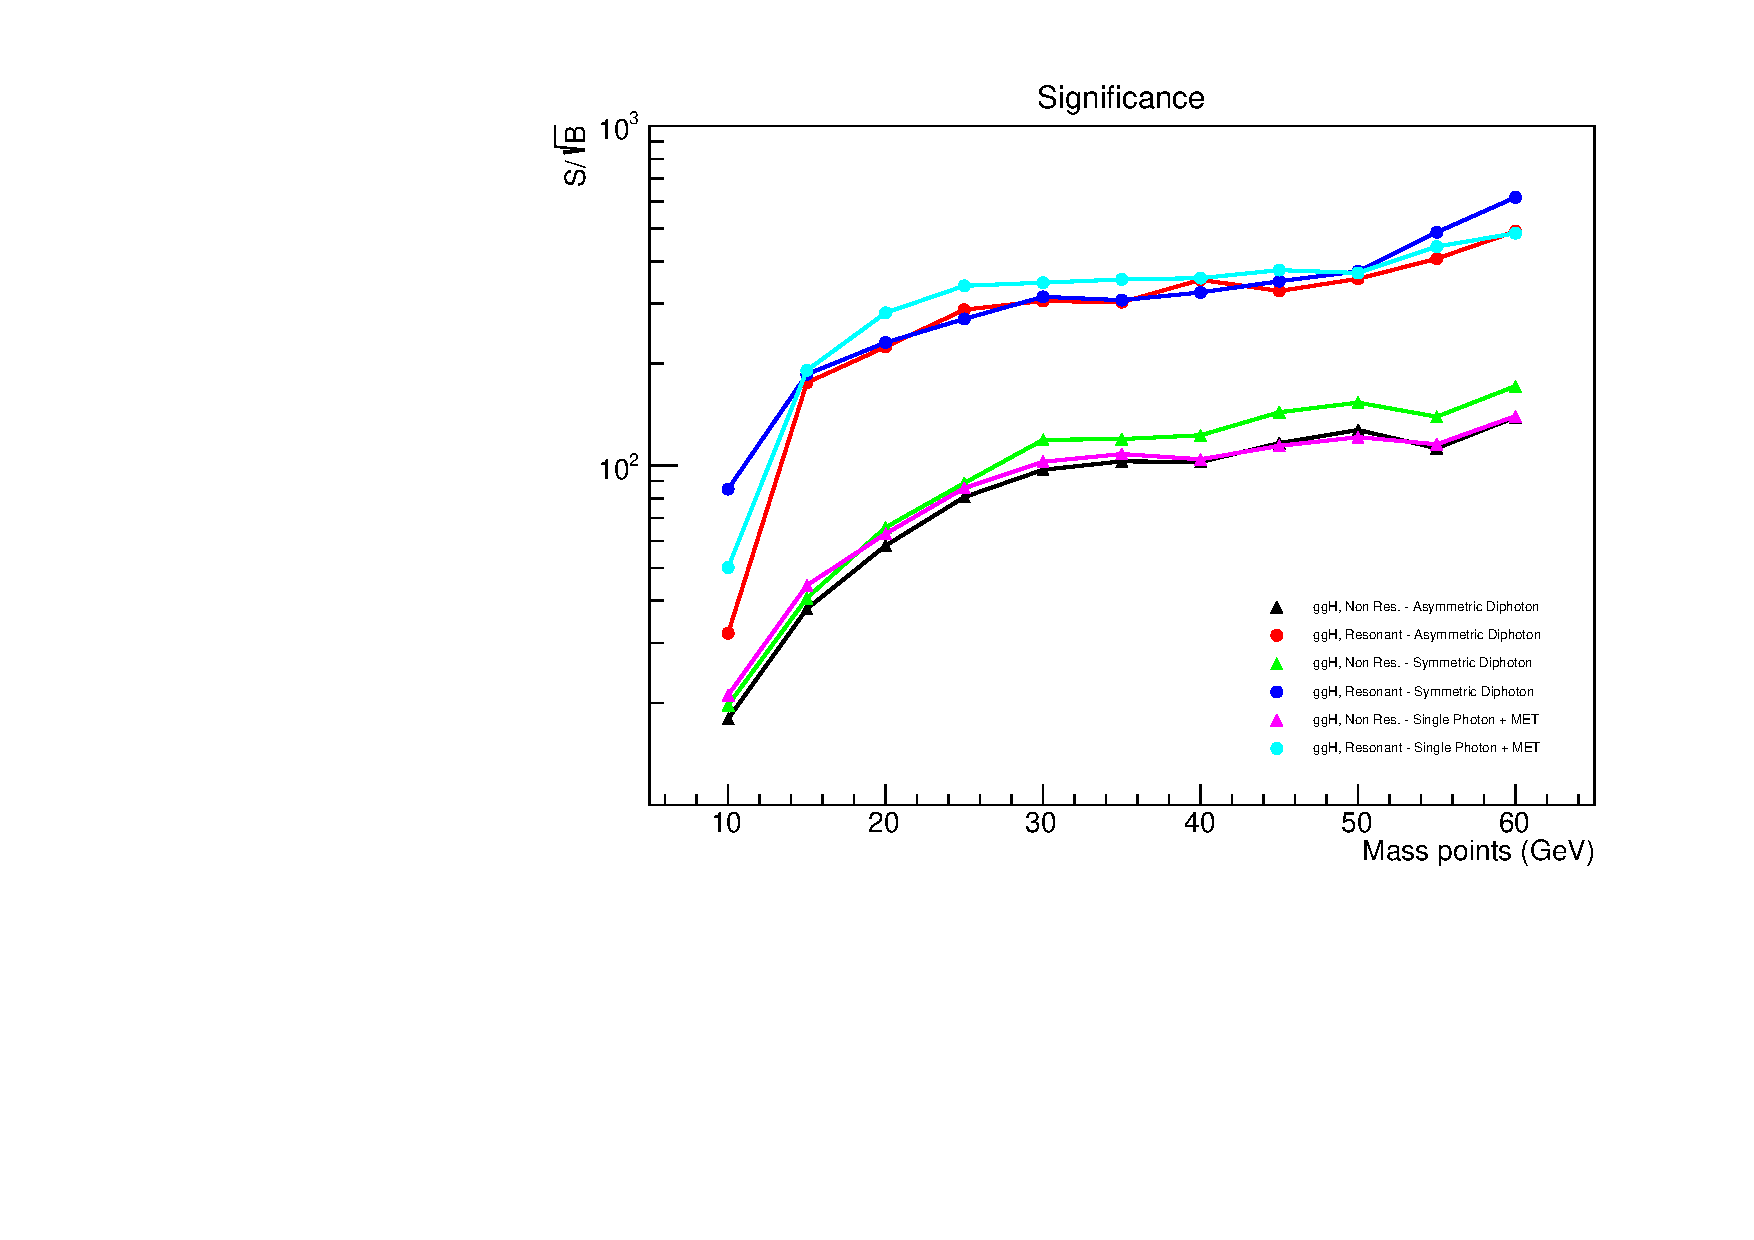
\includegraphics[width=0.45\textwidth]{triggerplots/Significance.pdf}
\caption{Signal efficiency (left) and significance (right) plots for different trigger scenarios in the gluon fusion analysis.}
\label{fig:triggers}
\end{figure}


Plots of some of the discriminating variables can be seen on subsection \ref{extrafigs} for both gluon fusion and ZH cases. The normalization reflects the expected number of events at $\sqrt{s} = 14 \TeV$ with a target luminosity of $100$ fb$^{-1}$. The distributions are shown after the full selection, without the transverse mass and $\Delta\phi(\gamma\gamma,\MET)$ cuts. For the ZH case, the plots are also before the $M_{T}(\gamma\gamma+\MET, \mu\mu)$ and $M(\mu\mu)$ cuts. For the gluon fusion channel, the single photon selection was used.


In Figure \ref{fig:branching_5sigma}, on the left, we show the branching ratio of $h\rightarrow\gamma\gamma+\MET$ needed for a significance of $5\sigma$, assuming the Standard Model Higgs cross subsection, for the gluon fusion analysis (assuming the $\gamma+\MET$ trigger strategy and selection). On the right, we show the branching ratio $h\rightarrow\gamma\gamma+\MET$ needed for a significance of $2\sigma$, which represents the $95\%$ confidence level for exclusion, assuming SM $ZH$ production. For the ZH case, we show the results for the strategies requiring at least one ($N(\gamma) \geq 1$) and at least two ($N(\gamma) \geq 2$) photons. %We assume the channel in which the Z decays to electrons to have efficiencies and background composition that are similar to the muon case, therefore, we multiply the significance by a factor of $1.4$ to obtain the full reach of the $Z\rightarrow ll$ channel.

%For the $ZH$ case, we also show the analysis strategy done by CMS for Run I, requiring only one photon. The selection on table \ref{tab:sel_all} remains the same, except for the subleading photon requirement and $M(\gamma\gamma)$ cut. Variables reconstructed with the diphoton information, such as $M_{T}(\gamma\gamma,\MET)$, are then reconstructed with the single photon information.

\subsubsection{Systematic Uncertainties}

While the uncertainties in the $ZH$ channel is expected to be dominated by statistics, the gluon fusion channel is very sensitive to the systematic uncertainties associated with the background predictions. We estimate the effect of these uncertainties by parametrizing the sensitivity as:
%
\begin{equation}
\mathcal{S}_{sys} = \frac{N_\text{Signal}}{\sqrt{N_\text{ Background}}+\sigma_{sys}\times N_\text{Background}},
\label{eqn:syst}
\end{equation}
%
with $\sigma_{sys}$ representing a source of uncertainty that does not scale with the amount of statistics.
%
%While the gluon fusion channel has higher sensitivity than the $ZH$ channel, the gluon fusion channel is more sensitive to systematic uncertainties, given the large amount of background events. 
%Because of that, the sensitivity could be easily degraded given large uncertainties on the background estimation methods. 
Figure \ref{fig:branching_5sigma} shows the effect on the $5\sigma$ branching ratios due to the addition of a $10\%$ systematic uncertainty according to Eqn \ref{eqn:syst}.

\begin{figure}[htbp]
\centering
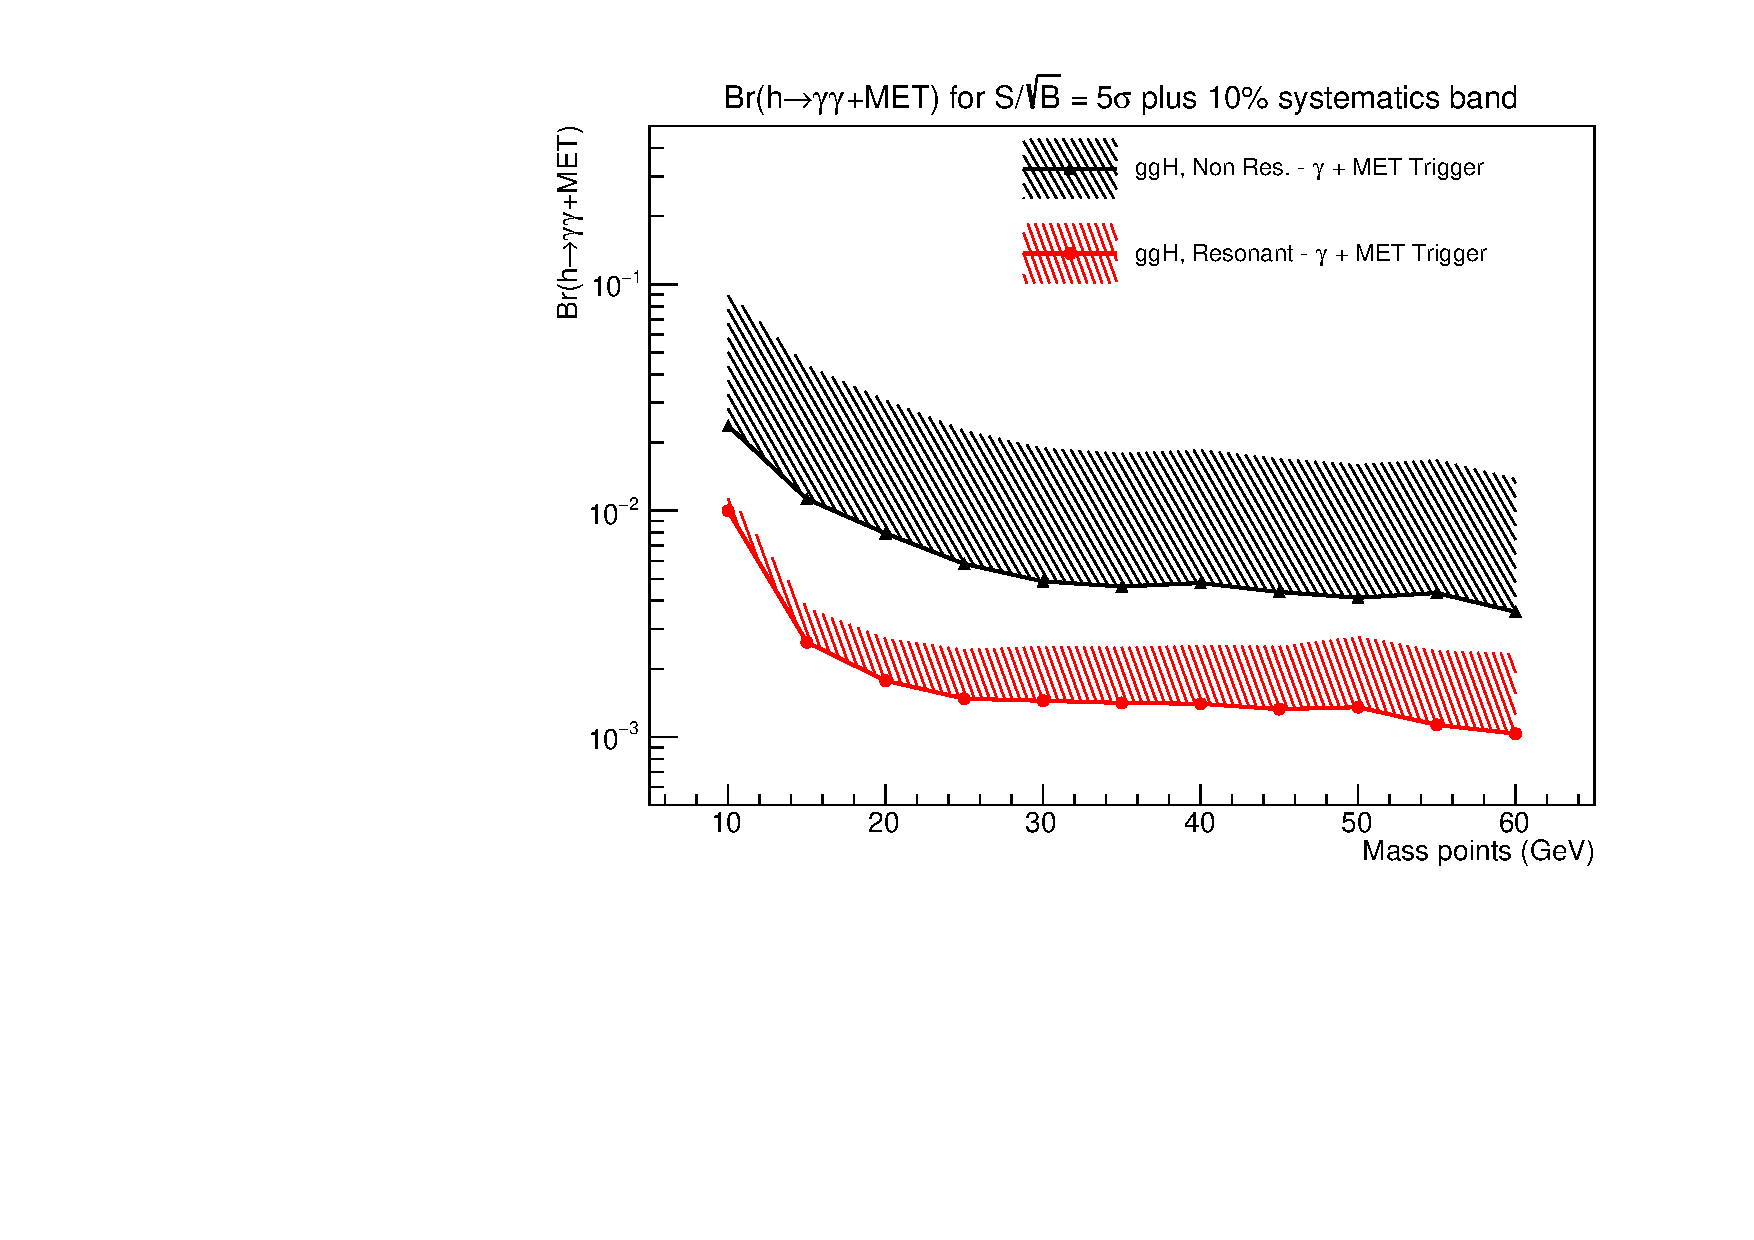
\includegraphics[width=0.45\textwidth]{finalresults/branchingratio_ggh.pdf}
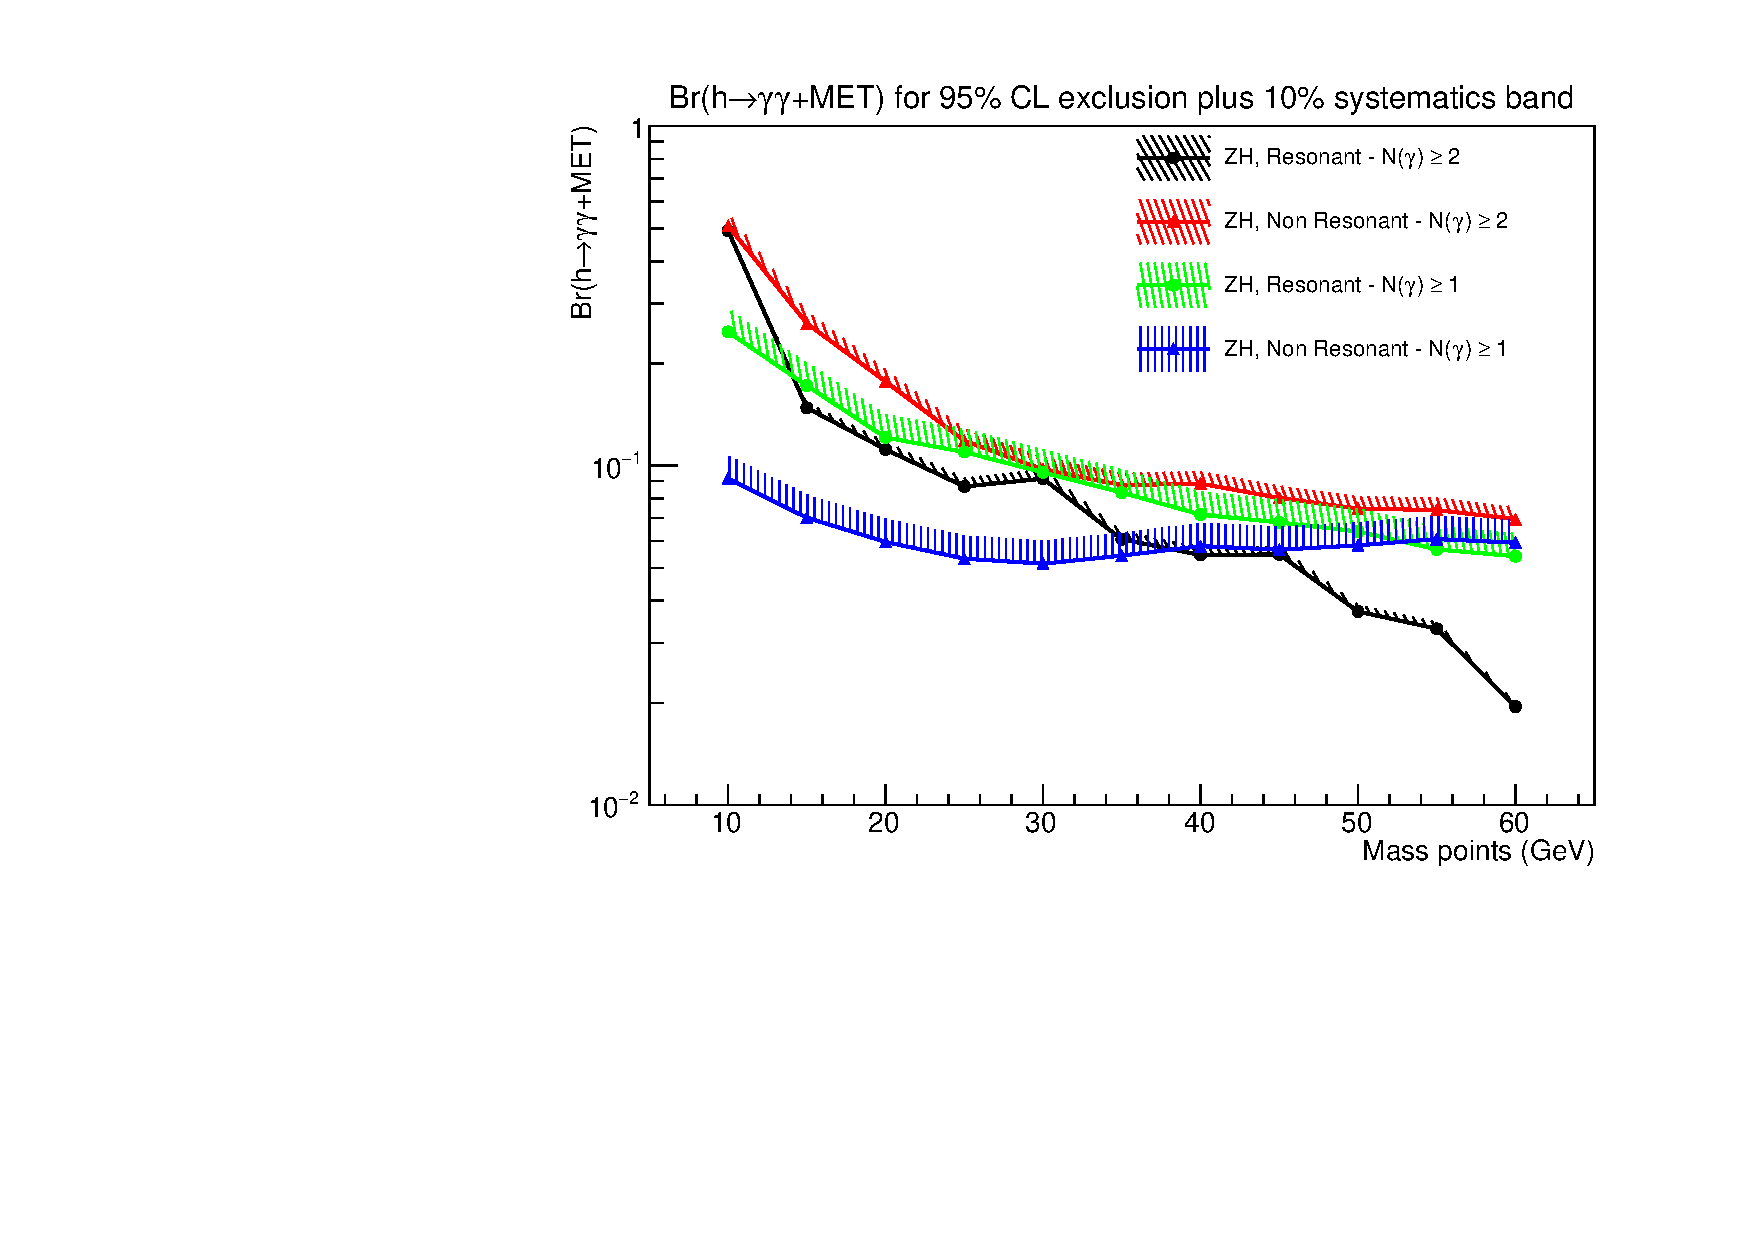
\includegraphics[width=0.45\textwidth]{finalresults/exclusion_zh.pdf}
\caption{(Left) $5\sigma$ branching ratios for the gluon fusion channel, for resonant and non-resonant final states, using the $\gamma+\MET$ trigger. (Right) Branching ratios for 95$\%$ confidence level exclusion in the ZH case, resonant and non-resonant topologies, requiring at least one photon ($N(\gamma) \geq 1$) and at least two photons ($N(\gamma) \geq 2$). The shaded areas correspond to a variation in systematics up to $10\%$.}
\label{fig:branching_5sigma}
\end{figure}
